%% LyX 2.3.6 created this file.  For more info, see http://www.lyx.org/.
%% Do not edit unless you really know what you are doing.
\documentclass[english]{article}
\usepackage[LGR,T1]{fontenc}
\usepackage[latin9]{inputenc}
\usepackage{float}
\usepackage{graphicx}

\makeatletter

%%%%%%%%%%%%%%%%%%%%%%%%%%%%%% LyX specific LaTeX commands.
\DeclareRobustCommand{\greektext}{%
  \fontencoding{LGR}\selectfont\def\encodingdefault{LGR}}
\DeclareRobustCommand{\textgreek}[1]{\leavevmode{\greektext #1}}
\ProvideTextCommand{\~}{LGR}[1]{\char126#1}

%% Because html converters don't know tabularnewline
\providecommand{\tabularnewline}{\\}
\floatstyle{ruled}
\newfloat{algorithm}{tbp}{loa}
\providecommand{\algorithmname}{Algorithm}
\floatname{algorithm}{\protect\algorithmname}

\makeatother

\usepackage{babel}
\begin{document}
\title{An improved Controlled Random Search method}
\author{Vasileios Charilogis$^{(1)}$, Ioannis G. Tsoulos$^{(1)}$, Alexandros
Tzallas,$^{(1)}$\\
Nikolaos Anastasopoulos$^{(2)}$}
\date{$^{(1)}$Department of Informatics and Telecommunications, University
of Ioannina, 47100 Arta, Greece \\
$^{(2)}$Department of Electrical and Computer Engineering, University
of Patras, Greece }
\maketitle
\begin{abstract}
A modified version of common global optimization method named Controlled
Random Search is presented here. The method aims to locate the global
minimum of multidimensional functions inside a rectangular hyperbox.
The new method modifies the original algorithm by incorporating a
new sampling method, a new termination rule and the periodical application
of local search optimization algorithm to the points sampled. The
new version is compared against the original one on a series of test
functions from the relevant literature and the results are reported.
\end{abstract}

\section{Introduction }

Global optimization\cite{GO1} is considered a problem of high complexity
with many applications. The problem is defined as the location of
the global minimum of a multi - dimensional function $f(x)$:
\begin{equation}
x^{*}=\mbox{arg}\min_{x\in S}f(x)\label{eq:eq1}
\end{equation}
Where $S\subset R^{n}$ is formulated as: 
\begin{equation}
S=\left[a_{1},b_{1}\right]\otimes\left[a_{2},b_{2}\right]\otimes\ldots\left[a_{n},b_{n}\right]\label{eq:eq2}
\end{equation}
 This problem is applicable in a wide range of areas such as physics
\cite{physics1,physics2}, chemistry \cite{chemistry1,chemistry2},
medicine \cite{med1,med2}, economics\cite{econ1} etc. In modern
theory there are two different categories of global optimization methods:
the stochastic methods and the deterministic methods.  The first category
contains the vast majority of methods such as Simulated Annealing
methods \cite{simann_major,simann1,simann2}, Genetic Algorithms \cite{ga1,ga2,ga3},
Tabu Search methods \cite{tabu1}, Particle Swarm Optimization \cite{pso_major,pso1,pso2}
etc. A common method that also belongs to stochastic methods is the
Controlled Random Search (CRS) method \cite{crs1}, which is a population
based algorithm. This method initially creates a set with randomly
selected points and repeatedly replaces the worst point in that set
with a randomly generated point and this process can continue until
some convergence criterion is met. The CRS method has been used intensively
in many problems such as geophysics problems \cite{crs_geophysics,crs_geophysics2},
optimal shape design problems \cite{crs_optimalshape1}, the animal
diet problem \cite{crs_animaldiet1}, the heat transfer problem \cite{crs_heat1}
etc. 

This CRS method has been thoroughly analyzed by many researchers in
the field such as the work A of Ali and Storey where two new variants
of the CRS method are proposed \cite{crs_modif0}. These variants
have proposed alternative techniques for the selection of the initial
sample set and usage of local search methods. Also, Pillo \emph{et
al} \cite{crs_modif1} suggested a hybrid CRS method where the base
algorithm is combined with a Newton - type unconstrained minimization
algorithm \cite{crs_newton} to enhance the efficiency of the method
in various test problems. Another work is of Kaelo and Ali , in which
they suggested \cite{crs_modif2} some modifications on the method
and especially in the new point generation step. Also, Filho and Albuquerque
have suggested \cite{crs_modif3} the usage of a distribution strategy
to accelerate the Controlled Random Search method. The current work
proposed three major modifications in the CRS method: a new point
replacement strategy, a stochastic termination rule and a periodical
application of some local search method. The first modification is
used to better explore the domain range of the function. The second
modification is made in order to achieve a better termination of the
method without wasting valuable computational time. The third modification
is used in order to speed up the method by applying a small amount
of steps of a local search method.

The rest of this article is organized as follows:\textbf{ }in Section
\ref{sec:Method-Description} the major steps of the CRS method as
well as the proposed modifications are outlined, in section \ref{sec:Experiments}
the results from the application of the proposed method on a series
of test functions are provided and finally in section \ref{sec:Conclusions}
some conclusions are presented.

\section{Method Description \label{sec:Method-Description}}

The Controlled Random Search has a series of steps that are described
in Algorithm \ref{alg:The-Controlled-Random}. The changes proposed
by the new method focus on three points:
\begin{enumerate}
\item \textgreek{T}he creation of a test point (\textbf{New\_Point} step)
is performed with a new technique described in subsection \ref{subsec:A-new-method}.
\item In the \textbf{Min\_Max} step the stochastic termination rule described
in subsection \ref{subsec:A-new-stopping} is used. The aim of this
rule is to terminate the method when, with some certainty, no lower
minimums are to be found. 
\item Apply a few steps of a local search procedure after \textbf{New\_Point}
step in the $\tilde{z}$ point. This procedure is used to bring the
test points closer to the corresponding minimums. This speeds up the
process of searching for new minima, although it obviously leads to
an increase in function calls 
\end{enumerate}
\begin{algorithm}
\caption{The Controlled Random Search algorithm.\label{alg:The-Controlled-Random}}

\begin{description}
\item [{Initialization}] Step:
\end{description}
\begin{enumerate}
\item \textbf{Se}t the value for the parameter $N$. A commonly used value
for that is $N=25n$.
\item \textbf{Set} a small positive value for $\epsilon$.
\item \textbf{Create} the set $T=\left\{ z_{1},z_{2},...,z_{N}\right\} $,
by randomly sampling $N$ points from $S$.
\end{enumerate}
\begin{description}
\item [{Min\_Max}] Step:
\end{description}
\begin{enumerate}
\item \textbf{Calculate} the points $z_{\mbox{min}}=\mbox{argmin}f(z)$
and $z_{\mbox{max}}=\mbox{argmax}f(z)$ and their function values
\[
f_{\mbox{max}}=\max_{z\in T}f(z)
\]
 and 
\[
f_{\mbox{min}}=\min_{z\in T}f(z)
\]
\item \textbf{If} $\left|f_{\mbox{max}}-f_{\mbox{min}}\right|<\epsilon$,
\textbf{then} \textbf{goto} \textbf{Local\_Search} Step.
\end{enumerate}
\begin{description}
\item [{New\_Point}] Step:
\end{description}
\begin{enumerate}
\item \textbf{Select} randomly the reduced set $\tilde{T}=\left\{ z_{T_{1}},z_{T_{2}},..,z_{T_{n+1}}\right\} $
from $T$.
\item \textbf{Compute} the centroid $G$: 
\[
G=\frac{1}{n}\sum_{i=1}^{n}z_{T_{i}}
\]
\item \textbf{Compute} a trial point $\tilde{z}=2G-z_{T_{n+1}}$.
\item \textbf{If} $\tilde{z}\ \notin S$ \textbf{or} $f(\tilde{z})\ge f_{\mbox{max}}$
\textbf{then} goto New\_Point step. 
\end{enumerate}
\begin{description}
\item [{Update}] Step:
\end{description}
\begin{enumerate}
\item $T=T\ \cup\{\tilde{z}\}-\left\{ z_{\mbox{max}}\right\} $.
\item \textbf{Goto Min\_Max} Step.
\end{enumerate}
\begin{description}
\item [{Local\_Search}] Step:
\end{description}
\begin{enumerate}
\item $z^{*}=\mbox{localSearch}(z)$.
\item Return the point $z^{*}$ as the discovered global minimum.
\end{enumerate}
\end{algorithm}


\subsection{A new method for trial points\label{subsec:A-new-method}}

The proposed technique to compute the trial point $\tilde{z}$ is
shown in Algorithm \ref{alg:newpoint}. According to this, the calculation
of the test point $\tilde{z}$ does not contain product with high
values as in the basic algorithm, so that the test point is not too
far from the centroid. This technique avoids vector jumps from the
centroid, where it has great gravity in the calculation for starting
the local optimization.

\begin{algorithm}

\caption{Proposed method to compute the trial point.\label{alg:newpoint}}

\begin{enumerate}
\item \textbf{Compute} the centroid $G$: 
\[
G=\frac{1}{n}\sum_{i=1}^{n}z_{T_{i}}
\]
\item Set $G=G+\frac{1}{n}z_{\mbox{min}}$
\item \textbf{Compute} a trial point $\tilde{z}=G-\frac{1}{n}z_{T_{n+1}}$.
\end{enumerate}
\end{algorithm}


\subsection{A new stopping rule \label{subsec:A-new-stopping}}

It is quite common in the optimization techniques to use a predefined
number of maximum iterations as the stopping rule of the method. Even
though this termination rule is easy to implement sometime could require
an excessive number of functions calls before termination and a more
sophisticated termination rule is needed.\textbf{ }The termination
rule proposed here is inspired from \cite{psotsoulos}. At every iteration
$k$ the variance\textbf{ $\sigma^{(k)}$ }of the quantity $f_{\mbox{min}}$
is calculated. If the optimization technique did not manage to find
a new estimation of the global minimum for some iterations, then it
is highly possible that the global minimum is already located and
hence the algorithm should terminate.\textbf{ }The termination rule
is defined as follows, terminate when 

\textbf{
\begin{equation}
\sigma^{(k)}\le\frac{\sigma^{\left(k_{\mbox{last}}\right)}}{2}\label{eq:termination_mine}
\end{equation}
}The term\textbf{ $k_{\mbox{last}}$ }represents the last iteration
where a new global minimum was located. 

\section{Experiments \label{sec:Experiments}}

\subsection{Test functions }

The modified version of the CRS was tested against the traditional
CRS on series of benchmark functions from the relevant literature
\cite{Ali1,Floudas1}. The following functions were used: 
\begin{itemize}
\item \textbf{Bf1} function. The function Bohachevsky 1 is given by the
equation
\end{itemize}
\[
f(x)=x_{1}^{2}+2x_{2}^{2}-\frac{3}{10}\cos\left(3\pi x_{1}\right)-\frac{4}{10}\cos\left(4\pi x_{2}\right)+\frac{7}{10}
\]
with $x\in[-100,100]^{2}$. 
\begin{itemize}
\item \textbf{Bf2} function. The function Bohachevsky 2 is given by the
equation 
\[
f(x)=x_{1}^{2}+2x_{2}^{2}-\frac{3}{10}\cos\left(3\pi x_{1}\right)\cos\left(4\pi x_{2}\right)+\frac{3}{10}
\]
with $x\in[-50,50]^{2}$. 
\item \textbf{Branin} function. The function is defined by $f(x)=\left(x_{2}-\frac{5.1}{4\pi^{2}}x_{1}^{2}+\frac{5}{\pi}x_{1}-6\right)^{2}+10\left(1-\frac{1}{8\pi}\right)\cos(x_{1})+10$
with $-5\le x_{1}\le10,\ 0\le x_{2}\le15$. The value of global minimum
is 0.397887.with $x\in[-10,10]^{2}$. 
\item \textbf{CM} function. The Cosine Mixture function is given by the
equation 
\[
f(x)=\sum_{i=1}^{n}x_{i}^{2}-\frac{1}{10}\sum_{i=1}^{n}\cos\left(5\pi x_{i}\right)
\]
with $x\in[-1,1]^{n}$. The value of the global minimum is -0.4 and
in our experiments we have used $n=4$.
\item \textbf{Camel} function. The function is given by 
\[
f(x)=4x_{1}^{2}-2.1x_{1}^{4}+\frac{1}{3}x_{1}^{6}+x_{1}x_{2}-4x_{2}^{2}+4x_{2}^{4},\quad x\in[-5,5]^{2}
\]
\item \textbf{Easom} function. The function is given by the equation 
\[
f(x)=-\cos\left(x_{1}\right)\cos\left(x_{2}\right)\exp\left(\left(x_{2}-\pi\right)^{2}-\left(x_{1}-\pi\right)^{2}\right)
\]
with $x\in[-100,100]^{2}.$ 
\item \textbf{Exponential} function. The function is given by 
\[
f(x)=-\exp\left(-0.5\sum_{i=1}^{n}x_{i}^{2}\right),\quad-1\le x_{i}\le1
\]
The global minimum is located at $x^{*}=(0,0,...,0)$ with value $-1$.
In our experiments we used this function with $n=2,4,8,16,32,64,100$
and the corresponding functions are denoted by the labels EXP2, EXP4,
EXP8, EXP16, EXP32, EXP64, EXP100.
\item \textbf{GoldStein \& Price }
\end{itemize}
\begin{eqnarray*}
f(x) & = & [1+(x_{1}+x_{2}+1)^{2}\\
 &  & (19-14x_{1}+3x_{1}^{2}-14x_{2}+6x_{1}x_{2}+3x_{2}^{2})]\times\\
 &  & [30+(2x_{1}-3x_{2})^{2}\\
 &  & (18-32x_{1}+12x_{1}^{2}+48x_{2}-36x_{1}x_{2}+27x_{2}^{2})]
\end{eqnarray*}

The function has 4 local minima in the range $[-2,2]^{2}$ and global
minimum $f^{*}=3.0$.
\begin{itemize}
\item \textbf{Griewank2} function. The function is given by
\[
f(x)=1+\frac{1}{200}\sum_{i=1}^{2}x_{i}^{2}-\prod_{i=1}^{2}\frac{\cos(x_{i})}{\sqrt{(i)}},\quad x\in[-100,100]^{2}
\]
The global minimum is located at the $x^{*}=(0,0,...,0)$ with value
0.
\item \textbf{Gkls} function. $f(x)=\mbox{Gkls}(x,n,w)$, is a function
with $w$ local minima, described in \cite{gkls} with $x\in[-1,1]^{n}$
and $n$ a positive integer between 2 and 100. The value of the global
minimum is -1 and in our experiments we have used $n=2,3$ and $w=50$.
The corresponding functions are denoted by the labels GKLS250 and
GKLS350. 
\item \textbf{Guilin Hills} function. $f(x)=3+\sum_{i=1}^{n}\left(c_{i}\frac{x_{i}+9}{x_{i}+10}\sin\left(\frac{\pi}{1-x_{i}+\frac{1}{2k_{i}}}\right)\right),\ x\in[0,1]^{n},\ c_{i}>0$
and $k_{i}$ being positive integers. The function has $\prod_{i=1}^{n}k_{i}$
local minima. In our experiments we have used $n=5,10$ and we set
the values of $k_{i}$ so that the number of minima was 50. The produced
functions are entitled GUILIN550 and GUILIN1050 in the result tables.
\item \textbf{Hansen} function. $f(x)=\sum_{i=1}^{5}i\cos\left[(i-1)x_{1}+i\right]\sum_{j=1}^{5}j\cos\left[(j+1)x_{2}+j\right]$,
$x\in[-10,10]^{2}$ . The global minimum of the function is -176.541793.
\item \textbf{Hartman 3} function. The function is given by
\[
f(x)=-\sum_{i=1}^{4}c_{i}\exp\left(-\sum_{j=1}^{3}a_{ij}\left(x_{j}-p_{ij}\right)^{2}\right)
\]
with $x\in[0,1]^{3}$ and $a=\left(\begin{array}{ccc}
3 & 10 & 30\\
0.1 & 10 & 35\\
3 & 10 & 30\\
0.1 & 10 & 35
\end{array}\right),\ c=\left(\begin{array}{c}
1\\
1.2\\
3\\
3.2
\end{array}\right)$ and
\[
p=\left(\begin{array}{ccc}
0.3689 & 0.117 & 0.2673\\
0.4699 & 0.4387 & 0.747\\
0.1091 & 0.8732 & 0.5547\\
0.03815 & 0.5743 & 0.8828
\end{array}\right)
\]
\item \textbf{Hartman 6} function.
\[
f(x)=-\sum_{i=1}^{4}c_{i}\exp\left(-\sum_{j=1}^{6}a_{ij}\left(x_{j}-p_{ij}\right)^{2}\right)
\]
with $x\in[0,1]^{6}$ and $a=\left(\begin{array}{cccccc}
10 & 3 & 17 & 3.5 & 1.7 & 8\\
0.05 & 10 & 17 & 0.1 & 8 & 14\\
3 & 3.5 & 1.7 & 10 & 17 & 8\\
17 & 8 & 0.05 & 10 & 0.1 & 14
\end{array}\right),\ c=\left(\begin{array}{c}
1\\
1.2\\
3\\
3.2
\end{array}\right)$ and
\[
p=\left(\begin{array}{cccccc}
0.1312 & 0.1696 & 0.5569 & 0.0124 & 0.8283 & 0.5886\\
0.2329 & 0.4135 & 0.8307 & 0.3736 & 0.1004 & 0.9991\\
0.2348 & 0.1451 & 0.3522 & 0.2883 & 0.3047 & 0.6650\\
0.4047 & 0.8828 & 0.8732 & 0.5743 & 0.1091 & 0.0381
\end{array}\right)
\]
\item \textbf{Rastrigin} function. The function is given by 
\[
f(x)=x_{1}^{2}+x_{2}^{2}-\cos(18x_{1})-\cos(18x_{2}),\quad x\in[-1,1]^{2}
\]
\item \textbf{\emph{Rosenbrock}}\emph{ function }\\
This function is given by 
\[
f(x)=\sum_{i=1}^{n-1}\left(100\left(x_{i+1}-x_{i}^{2}\right)^{2}+\left(x_{i}-1\right)^{2}\right),\quad-30\le x_{i}\le30.
\]
The global minimum is located at the $x^{*}=(0,0,...,0)$ with $f\left(x^{*}\right)=0$.
In our experiments we used this function with $n=20$.
\item \textbf{Shekel 7} function.
\end{itemize}
\[
f(x)=-\sum_{i=1}^{7}\frac{1}{(x-a_{i})(x-a_{i})^{T}+c_{i}}
\]

with $x\in[0,10]^{4}$ and $a=\left(\begin{array}{cccc}
4 & 4 & 4 & 4\\
1 & 1 & 1 & 1\\
8 & 8 & 8 & 8\\
6 & 6 & 6 & 6\\
3 & 7 & 3 & 7\\
2 & 9 & 2 & 9\\
5 & 3 & 5 & 3
\end{array}\right),\ c=\left(\begin{array}{c}
0.1\\
0.2\\
0.2\\
0.4\\
0.4\\
0.6\\
0.3
\end{array}\right)$. 
\begin{itemize}
\item \textbf{Shekel 5 }function.
\end{itemize}
\[
f(x)=-\sum_{i=1}^{5}\frac{1}{(x-a_{i})(x-a_{i})^{T}+c_{i}}
\]
 

with $x\in[0,10]^{4}$ and $a=\left(\begin{array}{cccc}
4 & 4 & 4 & 4\\
1 & 1 & 1 & 1\\
8 & 8 & 8 & 8\\
6 & 6 & 6 & 6\\
3 & 7 & 3 & 7
\end{array}\right),\ c=\left(\begin{array}{c}
0.1\\
0.2\\
0.2\\
0.4\\
0.4
\end{array}\right)$.
\begin{itemize}
\item \textbf{Shekel 10} function.
\end{itemize}
\[
f(x)=-\sum_{i=1}^{10}\frac{1}{(x-a_{i})(x-a_{i})^{T}+c_{i}}
\]
 

with $x\in[0,10]^{4}$ and $a=\left(\begin{array}{cccc}
4 & 4 & 4 & 4\\
1 & 1 & 1 & 1\\
8 & 8 & 8 & 8\\
6 & 6 & 6 & 6\\
3 & 7 & 3 & 7\\
2 & 9 & 2 & 9\\
5 & 5 & 3 & 3\\
8 & 1 & 8 & 1\\
6 & 2 & 6 & 2\\
7 & 3.6 & 7 & 3.6
\end{array}\right),\ c=\left(\begin{array}{c}
0.1\\
0.2\\
0.2\\
0.4\\
0.4\\
0.6\\
0.3\\
0.7\\
0.5\\
0.6
\end{array}\right)$. 
\begin{itemize}
\item \textbf{Sinusoidal} function. The function is given by 
\[
f(x)=-\left(2.5\prod_{i=1}^{n}\sin\left(x_{i}-z\right)+\prod_{i=1}^{n}\sin\left(5\left(x_{i}-z\right)\right)\right),\quad0\le x_{i}\le\pi.
\]
The global minimum is located at $x^{*}=(2.09435,2.09435,...,2.09435)$
with $f\left(x^{*}\right)=-3.5$. In our experiments we used $n=4,8,16,32$
and $z=\frac{\pi}{6}$ and the corresponding functions are denoted
by the labels SINU4, SINU8, SINU16, SINU32.
\item \textbf{Test2N} function. This function is given by the equation 
\[
f(x)=\frac{1}{2}\sum_{i=1}^{n}x_{i}^{4}-16x_{i}^{2}+5x_{i},\quad x_{i}\in[-5,5].
\]
The function has $2^{n}$ in the specified range and in our experiments
we used $n=4,5,6,7$. The corresponding values of global minimum is
-156.664663 for $n=4$, -195.830829 for $n=5$, -234.996994 for $n=6$
and -274.163160 for $n=7$.
\item \textbf{Test30N} function. This function is given by 
\[
f(x)=\frac{1}{10}\sin^{2}\left(3\pi x_{1}\right)\sum_{i=2}^{n-1}\left(\left(x_{i}-1\right)^{2}\left(1+\sin^{2}\left(3\pi x_{i+1}\right)\right)\right)+\left(x_{n}-1\right)^{2}\left(1+\sin^{2}\left(2\pi x_{n}\right)\right)
\]
with $x\in[-10,10]$. The function has $30^{n}$ local minima in the
specified range and we used $n=3,4$ in our experiments. The value
of global minimum for this function is 0.0
\end{itemize}

\subsection{Results}

In the experiments two different values were measured: the rejection
rate in the\textbf{ New\_Point} step and the average number of function
calls required. In the first case we measure the percentage of points
rejected during the\textbf{ New\_Point} step, i.e. points created
that are outside the domain range of the function. All the experiments
were conducted 30 times and different seed for the random number generator
was used each time. The local search method that used in the experiments
and denoted as localsearch(x), was a BFGS variant due to Powell\cite{powell}.
The experimental results are listed in Table \ref{tab:Experimenting-with-rejection}.
The column FUNCTION stands for the name of the objective function,
the column CRS-R represents the rejection rate\textbf{ }for the CRS
method while the column NEWCRS-R represents the same measure for the
proposed method. Similar, the column CRS-C represents the average
function calls for the CRS method and the column NEWCRS-C stands for
the average function calls of the proposed method. Also a statistical
comparison between the CRS and the proposed method is shown in Figure
\ref{fig:Statistical-comparison-for}.

The proposed method almost annihilates the rejection rate in every
test function. This is an evidence that the new mechanism proposed
here to create new point is more accurate than the traditional one.
Also, the proposed method requires lower number of function calls
than the CRS method as one can deduce from the relevant columns and
the statistical comparison.

\begin{table}
\caption{Experimenting with rejection rates.\label{tab:Experimenting-with-rejection}}

\begin{centering}
\begin{tabular}{|c|c|c|c|c|}
\hline 
FUNCTION & CRS-R & CRS-C & NEWCRS-R & NEWCRS-C\tabularnewline
\hline 
\hline 
BF1 & 1.37\% & 2523 & 0.00\% & 1689\tabularnewline
\hline 
BF2 & 1.33\% & 2506 & 0.17\% & 1569\tabularnewline
\hline 
BRANIN & 16.00\% & 2014 & 9.13\% & 851\tabularnewline
\hline 
CAMEL & 1.67\% & 2235 & 0.20\% & 1487\tabularnewline
\hline 
EASOM & 51.03\% & 591 & 11.43\% & 635\tabularnewline
\hline 
EXP2 & 3.03\% & 1290 & 0.70\% & 644\tabularnewline
\hline 
EXP4 & 2.67\% & 4688 & 0.00\% & 1302\tabularnewline
\hline 
EXP8 & 2.77\% & 16453 & 0.00\% & 2601\tabularnewline
\hline 
EXP16 & 4.00\% & 47400 & 0.00\% & 5207\tabularnewline
\hline 
EXP32 & 7.70\% & 93520 & 0.00\% & 10414\tabularnewline
\hline 
EXP64 & 18.80\% & 135638 & 0.00\% & 13602\tabularnewline
\hline 
EXP100 & 38.53\% & 129327 & 0.00\% & 14506\tabularnewline
\hline 
GKLS250 & 3.87\% & 1784 & 0.27\% & 1684\tabularnewline
\hline 
GKLS350 & 6.43\% & 3881 & 0.03\% & 2088\tabularnewline
\hline 
GOLDSTEIN & 3.60\% & 2154 & 0.70\% & 1829\tabularnewline
\hline 
GRIEWANK2 & 1.20\% & 2503 & 0.03\% & 2742\tabularnewline
\hline 
GUILIN550 & 8.33\% & 9129 & 0.00\% & 25333\tabularnewline
\hline 
GUILIN1050 & 9.63\% & 30806 & 0.00 & 10561\tabularnewline
\hline 
HANSEN & 47.60\% & 2643 & 4.03\% & 1736\tabularnewline
\hline 
HARTMAN3 & 9.97\% & 3009 & 6.13\% & 1331\tabularnewline
\hline 
HARTMAN6 & 13.37\% & 13615 & 0.00\% & 6091\tabularnewline
\hline 
RASTRIGIN & 9.17\% & 2130 & 1.33\% & 2986\tabularnewline
\hline 
ROSENBROCK & 0.00\% & 59024 & 0.00\% & 15719\tabularnewline
\hline 
SHEKEL5 & 4.73\% & 8974 & 0.00\% & 2967\tabularnewline
\hline 
SHEKEL7 & 3.70\% & 8606 & 0.00\% & 3236\tabularnewline
\hline 
SHEKEL10 & 2.73\% & 9264 & 0.00\% & 3479\tabularnewline
\hline 
SINU4 & 3.90\% & 6525 & 0.00\% & 2889\tabularnewline
\hline 
SINU8 & 5.10\% & 21561 & 0.00\% & 4946\tabularnewline
\hline 
SINU16 & 8.43\% & 62194 & 0.00\% & 9539\tabularnewline
\hline 
SINU32 & 14.40\% & 135986 & 0.00\% & 18456\tabularnewline
\hline 
TEST2N4 & 24.57\% & 10198 & 0.00\% & 3756\tabularnewline
\hline 
TEST2N5 & 34.17\% & 20850 & 0.00\% & 4806\tabularnewline
\hline 
TEST2N6 & 42.50\% & 43290 & 0.00\% & 6075\tabularnewline
\hline 
TEST2N7 & 50.37\% & 92658 & 0.00\% & 7005\tabularnewline
\hline 
TEST30N3 & 24.10\% & 4011 & 0.00\% & 5691\tabularnewline
\hline 
TEST30N4 & 27.30\% & 7432 & 0.00\% & 8579\tabularnewline
\hline 
\textbf{TOTAL} & \textbf{13.67\%} & 1000412 & \textbf{0.86\%} & 208031\tabularnewline
\hline 
\end{tabular}
\par\end{centering}
\end{table}
\begin{figure}
\caption{Statistical comparison for the function calls using box plots.\label{fig:Statistical-comparison-for}}

\begin{centering}
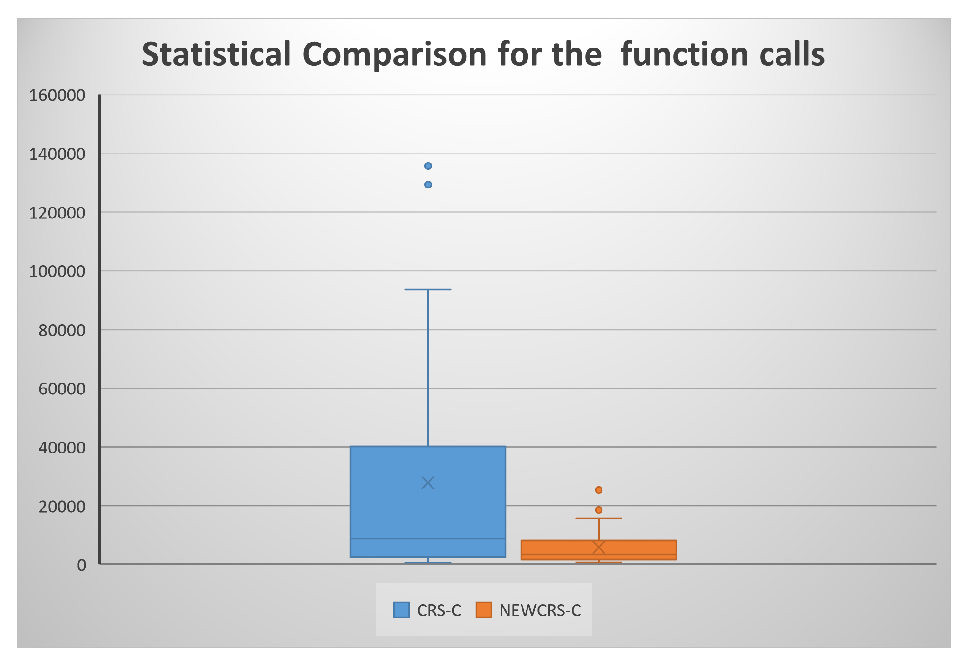
\includegraphics[scale=0.7]{values}
\par\end{centering}
\end{figure}


\section{Conclusions \label{sec:Conclusions}}

Three important modifications were proposed in the current work for
the CRS method. The first modification has to do with the new test
point generation process, which seems to be more accurate than the
original one. The new method almost every time creates points that
are within the domain range of the function. The second change adds
a new termination rule based on stochastic observations. The third
proposed modification applies a few steps of a local search procedure
to every trial point created by the algorithm. Judging by the results,
it seems that the proposed changes have two important effects. The
first is that the success of the algorithm in creating valid test
points is significantly improved. The second is the large reduction
in the number of function calls required to find the global minimum. 
\begin{thebibliography}{10}
\bibitem{GO1}T$\ddot{\mbox{o}}$rn A. and $\check{\mbox{Z}}$ilinskas
A., Global Optimization Volume 350 of Lecture Notes in Computer Science,
Springer, Heidelberg, 1987.

\bibitem{physics1}Patrice Ogou Yapo, Hoshin Vijai Gupta, Soroosh
Sorooshian, Multi-objective global optimization for hydrologic models,
Journal of Hydrology 204, pp. 83-97, 1998.

\bibitem{physics2}Q. Duan, S. Sorooshian, V. Gupta, Effective and
efficient global optimization for conceptual rainfall-runoff models,
Water Resources Research \textbf{28}, pp. 1015-1031 , 1992.

\bibitem{med1}Balsa-Canto E., Banga J.R., Egea J.A., Fernandez-Villaverde
A., de Hijas-Liste G.M. (2012) Global Optimization in Systems Biology:
Stochastic Methods and Their Applications. In: Goryanin I., Goryachev
A. (eds) Advances in Systems Biology. Advances in Experimental Medicine
and Biology, vol 736. Springer, New York, NY. https://doi.org/10.1007/978-1-4419-7210-1\_24

\bibitem{med2}P. Boutros, A. Ewing, K. Ellrott et al., Global optimization
of somatic variant identification in cancer genomes with a global
community challenge, Nat Genet \textbf{46}, pp. 318--319, 2014.

\bibitem{chemistry1}David J. Wales, Harold A. Scheraga, Global Optimization
of Clusters, Crystals, and Biomolecules, Science \textbf{27}, pp.
1368-1372, 1999. 

\bibitem{chemistry2}P.M. Pardalos, D. Shalloway, G. Xue, Optimization
methods for computing global minima of nonconvex potential energy
functions, Journal of Global Optimization \textbf{4}, pp. 117-133,
1994.

\bibitem{econ1}Zwe-Lee Gaing, Particle swarm optimization to solving
the economic dispatch considering the generator constraints, IEEE
Transactions on \textbf{18} Power Systems, pp. 1187-1195, 2003.

\bibitem{simann_major}S. Kirkpatrick, CD Gelatt, , MP Vecchi, Optimization
by simulated annealing, Science \textbf{220}, pp. 671-680, 1983.

\bibitem{simann1}L. Ingber, Very fast simulated re-annealing, Mathematical
and Computer Modelling \textbf{12}, pp. 967-973, 1989.

\bibitem{simann2}R.W. Eglese, Simulated annealing: A tool for operational
research, Simulated annealing: A tool for operational research \textbf{46},
pp. 271-281, 1990.

\bibitem{ga1}D. Goldberg, Genetic Algorithms in Search, Optimization
and Machine Learning, Addison-Wesley Publishing Company, Reading,
Massachussets, 1989.

\bibitem{ga2}Z. Michaelewicz, Genetic Algorithms + Data Structures
= Evolution Programs. Springer - Verlag, Berlin, 1996.

\bibitem{ga3}S.A. Grady, M.Y. Hussaini, M.M. Abdullah, Placement
of wind turbines using genetic algorithms, Renewable Energy \textbf{30},
pp. 259-270, 2005.

\bibitem{tabu1}A. Duarte, R. Mart�, F. Glover et al., Hybrid scatter
tabu search for unconstrained global optimization, Ann Oper Res \textbf{183},
pp. 95--123m, 2011.

\bibitem{pso_major}J. Kennedy and R. Eberhart, \textquotedbl Particle
swarm optimization,\textquotedbl{} Proceedings of ICNN'95 - International
Conference on Neural Networks, 1995, pp. 1942-1948 vol.4, doi: 10.1109/ICNN.1995.488968.

\bibitem{pso1}Riccardo Poli, James Kennedy kennedy, Tim Blackwell,
Particle swarm optimization An Overview, Swarm Intelligence \textbf{1},
pp 33-57, 2007. 

\bibitem{pso2}Ioan Cristian Trelea, The particle swarm optimization
algorithm: convergence analysis and parameter selection, Information
Processing Letters \textbf{85}, pp. 317-325, 2003.

\bibitem{crs1}W.L. Price, Global Optimization by Controlled Random
Search, Computer Journal \textbf{ 20}, pp. 367-370, 1977.

\bibitem{crs_geophysics}David N. Smith and John F. Ferguson, Constrained
inversion of seismic refraction data using the controlled random search,
Geophysics \textbf{65},pp. 1622-1630, 200.

\bibitem{crs_geophysics2}Cassiano Antonio Bortolozo, Jorge Lu�s Porsani,
Fernando Ac�cio Monteiro dos Santos, Emerson Rodrigo Almeida, VES/TEM
1D joint inversion by using Controlled Random Search (CRS) algorithm,
Journal of Applied Geophysics \textbf{112}, pp. 157-174, 2015.

\bibitem{crs_optimalshape1}J. Haslinger, D. Jedelsk�, T. Kozubek
et al, Genetic and Random Search Methods in Optimal Shape Design Problems,
Journal of Global Optimization \textbf{16}, pp. 109--131, 2000.

\bibitem{crs_animaldiet1}Radha Gupta, Manasa Chandan, Use of \textquotedblleft Controlled
Random Search Technique for Global Optimization\textquotedblright{}
in Animal Diet Problem, International Journal of Emerging Technology
and Advanced Engineering \textbf{3}, pp. 284-287, 2013.

\bibitem{crs_heat1}R.C. Mehta, S.B. Tiwari, Controlled random search
technique for estimation of convective heat transfer coefficient,
Heat Mass Transfer \textbf{43}, pp.1171--1177, 2007.

\bibitem{crs_modif0}M.M. Ali, C. Storey, Modified Controlled Random
Search Algorithms, International Journal of Computer Mathematics \textbf{53},
pp. 229-235, 1994.

\bibitem{crs_modif1}Di Pillo G., Lucidi S., Palagi L., Roma M. (1998)
A Controlled Random Search Algorithm with Local Newton-type Search
for Global Optimization. In: De Leone R., Murli A., Pardalos P.M.,
Toraldo G. (eds) High Performance Algorithms and Software in Nonlinear
Optimization. Applied Optimization, vol 24. Springer, Boston, MA.
https://doi.org/10.1007/978-1-4613-3279-4\_10

\bibitem{crs_newton}S. Lucidi, F. Rochetich, and M. Roma, Curvilinear
stabilization techniques for truncated Newton methods in large scale
unconstrained optimization, SIAM Journal on Optimization \textbf{8},
pp. 916--939, 1998.

\bibitem{crs_modif2}P. Kaelo, M.M. Ali, Some Variants of the Controlled
Random Search Algorithm for Global Optimization, Journal of Optimization
Theory and Applications \textbf{130}, pp. 253--264, 2006.

\bibitem{crs_modif3}Nelson Manzanares-filho , Rodrigo B. F. Albuquerque,
Accelerating Controlled Random Search Algorithms Using a Distribution
Strategy, In: EngOpt 2008 - International Conference on Engineering
Optimization, Rio de Janeiro, Brazil, 01 - 05 June 2008. 

\bibitem{psotsoulos}Ioannis G. Tsoulos, Modifications of real code
genetic algorithm for global optimization, Applied Mathematics and
Computation \textbf{203}, pp. 598-607, 2008.

\bibitem{Ali1}M. Montaz Ali, Charoenchai Khompatraporn, Zelda B.
Zabinsky, A Numerical Evaluation of Several Stochastic Algorithms
on Selected Continuous Global Optimization Test Problems, Journal
of Global Optimization \textbf{31}, pp 635-672, 2005. 

\bibitem{Floudas1}C.A. Floudas, P.M. Pardalos, C. Adjiman, W. Esposoto,
Z. G$\ddot{\mbox{u}}$m$\ddot{\mbox{u}}$s, S. Harding, J. Klepeis,
C. Meyer, C. Schweiger, Handbook of Test Problems in Local and Global
Optimization, Kluwer Academic Publishers, Dordrecht, 1999.

\bibitem{gkls}M. Gaviano, D.E. Ksasov, D. Lera, Y.D. Sergeyev, Software
for generation of classes of test functions with known local and global
minima for global optimization, ACM Trans. Math. Softw. \textbf{29},
pp. 469-480, 2003.

\bibitem{powell}M.J.D Powell, A Tolerant Algorithm for Linearly Constrained
Optimization Calculations, Mathematical Programming \textbf{45}, pp.
547-566, 1989. 
\end{thebibliography}

\end{document}
